\subsection{Exempelskript för ickelinjär kurvanpassning}
\label{sec:matlab-nonlinear}
Nedan finner ni ett Matlab skript ({\tt passning.m}) för incke linjär kurvanpassning.
Ekvationen som passas i exemplet är helt godtycklig:

\begin{equation}
  f(x) = a\frac{x^b+1}{x^{b+1}+1}
\end{equation}

\matlabcode{matlab/passning.m}

\pagebreak
När vi exekverar koden ovan får vi följande utdata i terminalen:

\begin{terminaloutput}
>> passning

fitobj = 

     General model:
     fitobj(x) = (a*(x.^b+1)./(x.^(b+1)+1))
     Coefficients (with 95% confidence bounds):
       a =       2.004  (1.988, 2.02)
       b =       3.207  (2.813, 3.601)
\end{terminaloutput}

samt att vi genererar \cref{fig:matlab}. Vi ser att passningen
lyckades och de sanna värdena ligger väl inom angivna 95\% 
konfidensintervall. Vi noterar dock att osäkerheten är relativt stor för
{\tt b}.

\begin{figure}
  \centering
  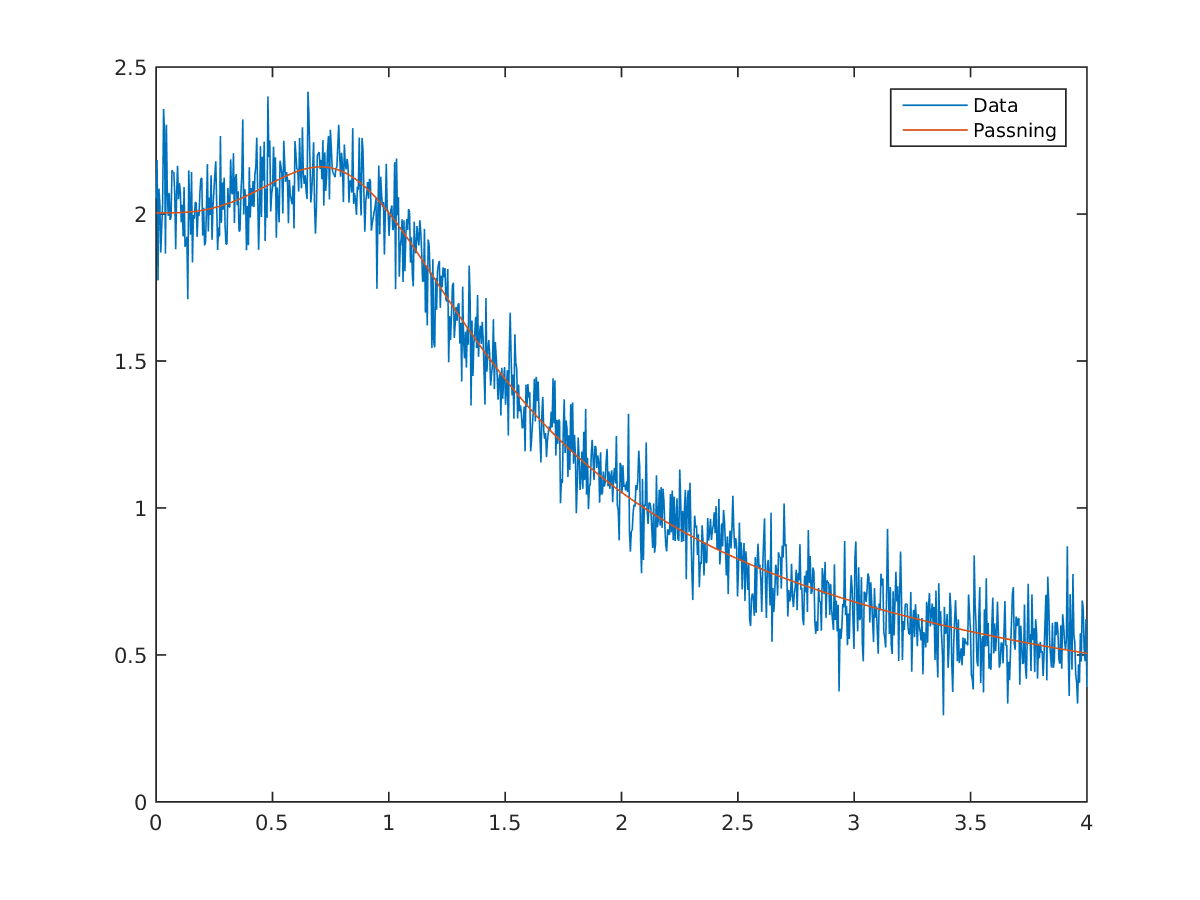
\includegraphics[scale=0.5]{matlab/passning.png}
  \caption{Ickelinjär kurvanpassning}
  \label{fig:matlab}
\end{figure}

